\documentclass[11pt,a4paper]{article}

%
%  Title:  "Do One Thing Well":
%          Unix Philosophy for AI Agent Skill Deck Architecture
%
%  An analysis of where the current protocol-enforcing skill deck falls short
%  in keeping the AI agent on-task, using correct skills consistently, avoiding
%  stale-data reliance, and ensuring full clean-room isolation through
%  scope-limited single-purpose sub-agents.
%

\usepackage{fontspec}
\usepackage{geometry}
\usepackage{booktabs}
\usepackage{longtable}
\usepackage{multicol}
\usepackage{enumitem}
\usepackage{xcolor}
\usepackage{listings}
\usepackage{tcolorbox}
\usepackage{hyperref}
\usepackage{fancyhdr}
\usepackage{titling}
\usepackage{abstract}
\usepackage{caption}
\usepackage{subcaption}
\usepackage{bytefield}
\usepackage{pgfplots}
\pgfplotsset{compat=1.18}
\usepackage{tikz}
\usetikzlibrary{
  arrows.meta,
  positioning,
  shapes.geometric,
  shapes.multipart,
  calc,
  chains,
  fit,
  matrix,
  backgrounds,
  decorations.pathreplacing,
  shadows.blur
}

\geometry{margin=1in, top=1.2in, bottom=1.2in}
\setmainfont{DejaVu Serif}
\setsansfont{DejaVu Sans}
\setmonofont{Hack}[Scale=0.88]

\definecolor{accentred}{HTML}{D64045}
\definecolor{accentgreen}{HTML}{2E7D32}
\definecolor{accentblue}{HTML}{1565C0}
\definecolor{accentyellow}{HTML}{F9A825}
\definecolor{accentpurple}{HTML}{7B1FA2}
\definecolor{accentgray}{HTML}{616161}
\definecolor{bglight}{HTML}{F5F5F5}
\definecolor{borderlight}{HTML}{BDBDBD}
\definecolor{codebg}{HTML}{ECEFF1}

\hypersetup{
  colorlinks=true,
  linkcolor=accentblue,
  urlcolor=accentpurple,
  citecolor=accentgreen
}

\pagestyle{fancy}
\fancyhf{}
\fancyhead[L]{\small\textit{Unix Philosophy for AI Agent Skill Deck Architecture}}
\fancyhead[R]{\small\thepage}
\renewcommand{\headrulewidth}{0.4pt}

\tcbuselibrary{skins, breakable}

\newtcolorbox{quotebox}{
  colback=bglight,
  colframe=borderlight,
  boxrule=0.5pt,
  arc=4pt,
  left=12pt,
  right=12pt,
  top=8pt,
  bottom=8pt,
  before skip=10pt,
  after skip=10pt,
  fontupper=\itshape\small
}

\newtcolorbox{gapbox}{
  colback=accentred!5,
  colframe=accentred!70,
  boxrule=0.8pt,
  arc=4pt,
  left=12pt,
  right=12pt,
  top=8pt,
  bottom=8pt,
  before skip=8pt,
  after skip=8pt,
  fontupper=\small
}

\newtcolorbox{strengthbox}{
  colback=accentgreen!5,
  colframe=accentgreen!70,
  boxrule=0.8pt,
  arc=4pt,
  left=12pt,
  right=12pt,
  top=8pt,
  bottom=8pt,
  before skip=8pt,
  after skip=8pt,
  fontupper=\small
}

\newtcolorbox{insightbox}{
  colback=accentblue!5,
  colframe=accentblue!70,
  boxrule=0.8pt,
  arc=4pt,
  left=12pt,
  right=12pt,
  top=8pt,
  bottom=8pt,
  before skip=8pt,
  after skip=8pt,
  fontupper=\small
}

\lstdefinestyle{pseudocode}{
  backgroundcolor=\color{codebg},
  basicstyle=\small\ttfamily,
  frame=single,
  rulecolor=\color{borderlight},
  framesep=8pt,
  xleftmargin=12pt,
  xrightmargin=12pt,
  aboveskip=10pt,
  belowskip=10pt,
  numbers=none,
  breaklines=true,
  postbreak=\mbox{\textcolor{accentgray}{$\hookrightarrow$}\space}
}

\lstdefinestyle{bashstyle}{
  backgroundcolor=\color{codebg},
  basicstyle=\small\ttfamily,
  frame=single,
  rulecolor=\color{borderlight},
  framesep=8pt,
  xleftmargin=12pt,
  xrightmargin=12pt,
  aboveskip=10pt,
  belowskip=10pt,
  numbers=none,
  breaklines=true
}

\renewcommand{\abstractnamefont}{\normalfont\large\bfseries}
\renewcommand{\abstracttextfont}{\normalfont\normalsize}

\title{\textbf{``Do One Thing Well''}\\[6pt]
       \large Unix Philosophy as a Design Framework for\\[4pt]
       AI Agent Skill Deck Architecture}
\author{
  \begin{tabular}{c}
  \textbf{Michael Conrad}\\[2pt]
  \small Investigation Direction \& Review\\[8pt]
  \textbf{with OpenCode (deepseek-v4-pro)}\\[2pt]
  \small Research \& Composition
  \end{tabular}
}
\date{May 2026}

\begin{document}

\maketitle

\vspace{-12pt}
{\small
\hspace*{\fill}%
\begin{minipage}{0.92\textwidth}
\textit{Note on authorship.}\ \ Research, analysis, and manuscript composition were performed by \textbf{OpenCode (deepseek-v4-pro)}, an AI agent, under the direction of Michael Conrad.  Conrad designed the investigation scope, reviewed the findings, evaluated the conclusions through iterative discourse with the agent, and approved the final text.  The skill deck under analysis is a design artifact created under Conrad's direction and refined through the same discourse process.
\end{minipage}%
\hspace*{\fill}%
}
\vspace{12pt}

\begin{abstract}
\noindent
Modern AI coding agents are converging on structured skill-deck architectures---curated collections of capabilities, instructions, and tools that agents invoke to perform complex software engineering tasks.  The opencode-config skill deck represents the most architecturally ambitious implementation surveyed: a protocol-enforcing agent operating system with 45 skills, 237 task files, a fixed dispatch-chain pipeline, pipeline-scoped authorization, tiered mandates, and a pure-orchestrator sub-agent model.  This paper maps the skill deck against the Unix philosophy of \emph{``do one thing well''} and the extensive academic literature on agent skill systems, identifying where the current architecture succeeds, where it falls short, and what structural changes would bring it into alignment with both the Unix design tradition and the emerging research consensus.  We find that while the deck's theoretical foundations are uniquely strong among surveyed systems, its \emph{implementation} suffers from text-bloat (163K words of guidelines and skills), inconsistent trigger semantics, and incomplete clean-room enforcement---all of which produce exactly the agent misbehavior (skill confusion, stale-data reliance, premature completion claims) that the architecture was designed to prevent.
\end{abstract}

\tableofcontents
\newpage

%=====================================================================
\section{Introduction}

The Unix philosophy, articulated by Doug McIlroy in 1978 and refined through four decades of systems design, rests on a small set of principles: (1) make each program do one thing well, (2) expect the output of every program to become the input to another, (3) design programs to be used with other programs, (4) use text streams as the universal interface, and (5) build prototypes early and iterate.\footnote{McIlroy, M.~D., Pinson, E.~N., \& Tague, B.~A.  ``Unix Time-Sharing System: Forward.'' \emph{The Bell System Technical Journal}, 57(6), 1978.}

These principles were devised for operating-system processes communicating through pipes.  Remarkably, they map onto the emerging field of AI agent architecture with surprising fidelity~\cite{piskala2026unix}.  A skill is a ``program'' that does one thing well.  Sub-agents are ``processes'' connected by structured result contracts (``pipes'').  The orchestrator is a ``shell'' that composes them.

The opencode-config skill deck implements a protocol-enforcing agent operating system: a structured hierarchy of guidelines, skills, and tasks designed to govern an AI agent's behavior through every stage of the software development lifecycle.  At 163,000 words across 282 discrete files, it is the largest and most architecturally rigorous skill deck we have encountered in our survey of over 30 agent systems and 15 academic papers.

\begin{quotebox}
\textbf{Research methodology.}  This paper is based on two rounds of exhaustive parallel research.  Round 1 surveyed 25+ production agent systems (Claude Code, OpenAI Codex, GitHub Copilot, Cursor, Windsurf Cascade, CrewAI, AutoGen, Aider, Goose, Sweep, MetaGPT, Devin, Amazon Q Developer, JetBrains Junie, Tabnine, and others).  Round 2 analyzed 13 academic papers (arXiv, ACL, NeurIPS venues) and 4 major industry essays on agent architecture.  All claims about external systems are sourced from publicly available documentation and peer-reviewed literature.
\end{quotebox}

The central question this paper addresses is: \textbf{where does the current skill deck fall short of its own design goals, and what would a Unix-philosophy-aligned version look like?}

\newpage

%=====================================================================
\section{Current Architecture}

\subsection{Structural Overview}

The skill deck implements a three-tier hierarchy (Table~\ref{tab:tiers}) and a fixed dispatch chain (Figure~\ref{fig:pipeline}):

\begin{table}[htbp]
\centering
\caption{Skill Deck Layer Hierarchy}
\label{tab:tiers}
\begin{tabular}{@{}llrl@{}}
\toprule
\textbf{Layer}    & \textbf{Directory}                & \textbf{Files} & \textbf{Words} \\
\midrule
Guidelines        & \texttt{.opencode/guidelines/}    & 26             & 66,908          \\
Skills (SKILL.md) & \texttt{.opencode/skills/*/}      & 45             & 96,038          \\
Tasks             & \texttt{.opencode/skills/*/tasks/}& 237            & ---             \\
\bottomrule
\end{tabular}
\end{table}

\begin{figure}[htbp]
\centering
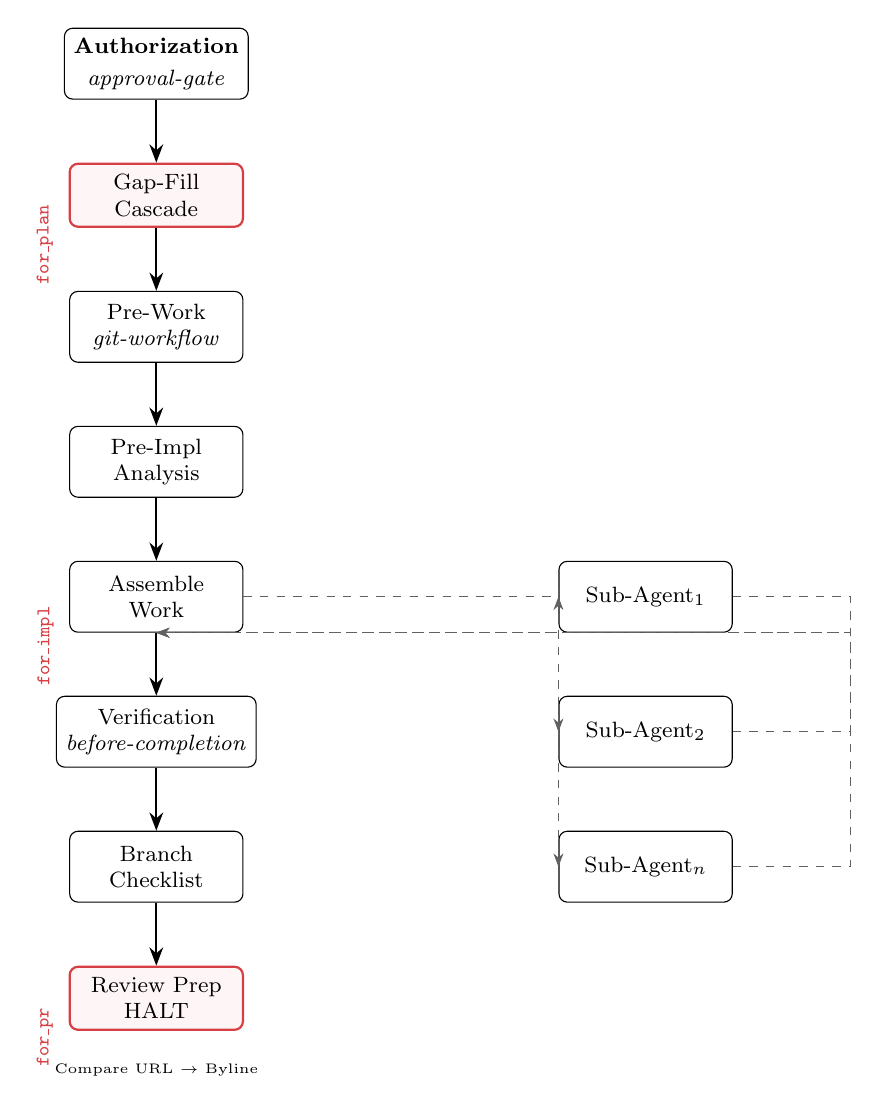
\begin{tikzpicture}[
  node distance=8mm and 5mm,
  box/.style={
    draw, rounded corners=3pt, minimum width=2.2cm, minimum height=0.9cm,
    align=center, font=\footnotesize, fill=white,
  },
  gate/.style={
    draw=accentred, rounded corners=3pt, minimum width=2.2cm, minimum height=0.8cm,
    align=center, font=\footnotesize, fill=accentred!5, thick,
  },
  arrow/.style={->, >=Stealth, thick},
  sub/.style={->, >=Stealth, dashed, draw=accentgray},
]

\node[box] (auth) {\textbf{Authorization}\\[2pt]\textit{approval-gate}};
\node[gate, below=of auth] (gap) {Gap-Fill\\Cascade};
\node[box, below=of gap] (pw) {Pre-Work\\\textit{git-workflow}};
\node[box, below=of pw] (pia) {Pre-Impl\\Analysis};
\node[box, below=of pia] (dac) {Assemble\\Work};
\node[box, right=4cm of dac] (sa1) {Sub-Agent$_1$};
\node[box, below=of sa1] (sa2) {Sub-Agent$_2$};
\node[box, below=of sa2] (san) {Sub-Agent$_n$};
\node[box, below=of dac] (vbc) {Verification\\\textit{before-completion}};
\node[box, below=of vbc] (fb) {Branch\\Checklist};
\node[gate, below=of fb] (rp) {Review Prep\\HALT};

\draw[arrow] (auth) -- (gap);
\draw[arrow] (gap) -- (pw);
\draw[arrow] (pw) -- (pia);
\draw[arrow] (pia) -- (dac);
\draw[sub] (dac.east) -| (sa1.west);
\draw[sub] (dac.east) -| (sa2.west);
\draw[sub] (dac.east) -| (san.west);
\draw[sub] (sa1.east) -- ++(1.5,0) |- (dac.south);
\draw[sub] (sa2.east) -- ++(1.5,0) |- (dac.south);
\draw[sub] (san.east) -- ++(1.5,0) |- (dac.south);
\draw[arrow] (dac) -- (vbc);
\draw[arrow] (vbc) -- (fb);
\draw[arrow] (fb) -- (rp);

\node[font=\tiny, align=center, below=0.3cm of rp] {Compare URL $\to$ Byline};

% scope boundary annotations
\node[font=\scriptsize, rotate=90, anchor=west, accentred, left=0.3cm of gap] {\texttt{for\_plan}};
\node[font=\scriptsize, rotate=90, anchor=west, accentred, left=0.3cm of dac] {\texttt{for\_impl}};
\node[font=\scriptsize, rotate=90, anchor=west, accentred, left=0.3cm of rp] {\texttt{for\_pr}};

\end{tikzpicture}
\caption{The Fixed Dispatch Chain.  Sub-agents spawn in parallel from the Assembly stage and return structured result contracts.  Scope boundaries enforce hard halts.}
\label{fig:pipeline}
\end{figure}

\subsection{Key Innovations}

The skill deck makes five architectural contributions that have no equivalent in any surveyed system:

\begin{strengthbox}
\textbf{(1) Pure Orchestrator.}  The main agent is a stateless router that never loads implementation context, never edits files, and never performs analysis inline.  Every operation is a sub-agent dispatch.  This is enforced as a Tier~1 critical violation with zero exceptions.  Cursor's own research validated the opposite approach---they found their ``integrator'' role (central quality control) became a bottleneck and had to be removed.\footnote{Cursor Engineering Blog.  ``Scaling Agents.''  April 2026.  Their alternative was recursive planner-worker hierarchies without a central integrator; this deck achieves the same result through mandatory sub-agent dispatch.}
\end{strengthbox}

\begin{strengthbox}
\textbf{(2) Pipeline-Scoped Authorization.}  Authorization is a continuum with deterministic parsing.  \texttt{"approved \#N"} (bare) $\to$ \texttt{standard} (halt at review-prep).  \texttt{"approved \#N to PR"} $\to$ \texttt{for\_pr} (full pipeline with auto-PR).  A verb-prefix table maps every phrase deterministically.  Hard HALT at the scope boundary is enforced.  No other system has pipeline-stage authorization.
\end{strengthbox}

\begin{strengthbox}
\textbf{(3) Tiered Mandate System.}  Rules are classified by override eligibility.  Tier~1 mandates (branch protection, worktree requirement, no \texttt{/tmp/}, human-only merge) never yield to developer authorization.  Tier~2 mandates (spec-before-code, plan-before-implementation) can be waived with explicit authorization.  No other system classifies constraints by this dimension.
\end{strengthbox}

\begin{strengthbox}
\textbf{(4) Tool-Call Evidence Requirement.}  Every verification claim must reference a tool-call artifact produced in the current session.  ``No tool-call artifact = the claim is forbidden.''  This is a structural gate, not a suggestion.  CrewAI's guardrails come closest but operate as validation functions returning pass/fail---they do not require evidence artifacts.
\end{strengthbox}

\begin{strengthbox}
\textbf{(5) Plan-Bridge Hierarchy.}  Spec $\to$ Plan $\to$ Sub-issues with formal \texttt{github\_sub\_issue\_write} linkage and phase-count cross-reference verification.  Plan body phase count must match \texttt{get\_sub\_issues} count before implementation proceeds.  No other system enforces count-level structural verification.
\end{strengthbox}

\newpage

%=====================================================================
\section{What the Research Says}

\subsection{Convergence: The Industry Is Moving Here}

Three patterns have become broadly adopted across the industry during 2025--2026:

\begin{enumerate}[leftmargin=*]
  \item \textbf{The Agent Skills specification} (\texttt{agentskills.io}).  Originally developed by Anthropic, adopted by 30+ clients including Claude Code, Gemini CLI, OpenCode, Cursor, GitHub Copilot, VS Code, OpenAI Codex, Junie, Goose, and Qodo.  SKILL.md with progressive disclosure is becoming a de facto standard.\footnote{\url{https://agentskills.io/specification}}
  \item \textbf{Progressive disclosure.}  Skills load only \texttt{name} + \texttt{description} into the system prompt; full content loads only on invocation.  Every system surveyed uses this pattern.
  \item \textbf{Sub-agent context isolation.}  Spawning separate agents with their own context windows, returning summaries only.  Universal across Claude Code, OpenAI, GitHub Copilot, and Goose.
\end{enumerate}

\subsection{Research Validation of the Deck's Design Choices}

The academic literature from 2024--2026 strongly supports the deck's architectural direction (Table~\ref{tab:validation}).

\begin{table}[htbp]
\centering
\caption{Research Validation of Deck Design Choices}
\label{tab:validation}
\small
\begin{tabular}{@{}p{3.5cm}p{5cm}p{5cm}@{}}
\toprule
\textbf{Design Choice} & \textbf{Supporting Evidence} & \textbf{Source} \\
\midrule
Structured pipeline $>$ free-form conversation
  & CAID: +26.7\% absolute improvement; Anthropic ``Building Effective Agents'' recommends workflows for production
  & Geng \& Neubig (arXiv:2603.21489); \cite{anthropic2024agents} \\
\midrule
Orchestrator purity
  & AgentSpawn: 34\% higher completion with pure orchestration; Small Model as Master Orchestrator paper
  & Costa (arXiv:2602.07072); \cite{smallorchestrator2026} \\
\midrule
Fewer, better skills
  & GraSP: focused 2--3 skills outperform comprehensive libraries; excessive skills actively hurt
  & Xia et al. (arXiv:2604.17870) \\
\midrule
Clean-room verification
  & ChemCrow: LLM-based self-evaluation fundamentally unreliable; producer cannot also verify
  & Multiple papers: ChemCrow, NL2Repo-Bench, PR rejection study \\
\midrule
Verification gates between stages
  & NeuroClaw: checkpointing + post-execution verification; Dual-State Architecture: deterministic guards necessary
  & arXiv:2604.24696; Thompson (arXiv:2512.20660) \\
\midrule
Architecture $>$ model capability
  & Debug2Fix: weaker models with better tool design match stronger models
  & Garg \& Huang (arXiv:2602.18571) \\
\midrule
Curated skills $>$ generated skills
  & SoK: self-generated skills actively degrade performance; 26.1\% of community skills contain vulnerabilities
  & Jiang et al. (arXiv:2602.20867); Xu \& Yan (arXiv:2602.12430) \\
\bottomrule
\end{tabular}
\end{table}

\subsection{Documented Failure Modes}

The research literature also identifies specific failure patterns that are \emph{not} fully addressed by the current deck implementation (Table~\ref{tab:failures}).  These form the basis for our gap analysis in \S\ref{sec:gaps}.

\begin{table}[htbp]
\centering
\caption{Agent Failure Modes from the Literature}
\label{tab:failures}
\small
\begin{tabular}{@{}p{4cm}p{4cm}p{5cm}@{}}
\toprule
\textbf{Failure Mode} & \textbf{Deck Has Rule?} & \textbf{Is Rule Actually Enforced?} \\
\midrule
Context pollution (stale state fills window)               & Yes (pure orchestrator) & \textbf{Partial}---guideline text can still leak \\
\midrule
Skill overload degrades performance                        & Yes (trigger-based routing) & \textbf{Partial}---trigger keywords ambiguous \\
\midrule
Agent self-verification is unreliable                      & Yes (clean-room dispatch) & \textbf{Partial}---no audit trail of exclusions \\
\midrule
Guardrail bypass via chain-of-thought                      & Yes (Tier~1 mandates) & \textbf{Partial}---text-based, not structural \\
\midrule
Premature completion claims (metadata-as-evidence)         & Yes (verification-before-completion) & \textbf{Partial}---gap-fill cascade can skip \\
\midrule
Confirmation-as-authorization rationalization              & Yes (explicit tiered model) & \textbf{Partial}---edge-case phrases ambiguous \\
\midrule
Skill interference / routing failures                      & Yes (trigger-based) & \textbf{Weak}---no conflict detection \\
\midrule
Approval fatigue (rubber-stamping)                         & N/A (pipeline-scoped) & \textbf{N/A}---but scope-granularity unverified \\
\midrule
Overtriggering subagents (skill escalation language)       & No explicit rule & \textbf{No}---escalation language embedded \\
\midrule
Long-horizon coherence loss (cross-file fragility)         & Yes (work state file) & \textbf{Partial}---context leaks between phases \\
\bottomrule
\end{tabular}
\end{table}

\newpage

%=====================================================================
\section{The Unix Philosophy Framework}

\subsection{Mapping Unix Principles to Agent Architecture}

Table~\ref{tab:unix} maps the five canonical Unix principles onto AI agent skill deck design.

\begin{table}[htbp]
\centering
\caption{Unix-to-Agent Architecture Mapping}
\label{tab:unix}
\small
\begin{tabular}{@{}p{3.5cm}p{5cm}p{5cm}@{}}
\toprule
\textbf{Unix Principle}       & \textbf{Agent Architecture Analog}          & \textbf{Current Implementation} \\
\midrule
1. Do one thing well
  & Each skill handles exactly one concern; single-purpose sub-agents
  & SCP codified in critical rules; 45 skills exist; \textbf{BUT} many skills exceed the 3,000-word atomicity threshold \\
\midrule
2. Output of one $\to$ input of another
  & Structured result contracts between sub-agents and orchestrator
  & Result contracts specified but \textbf{NOT universally enforced}; some skills lack contract schemas \\
\midrule
3. Designed to be used with other programs
  & Skills composable into pipeline stages; DAG orchestration
  & Fixed dispatch chain hardcoded; \textbf{NO DAG composition model} \\
\midrule
4. Text streams as universal interface
  & Markdown / YAML as interchange; tool-call evidence artifacts
  & Evidence artifacts required but \textbf{NO common schema for artifact interchange} \\
\midrule
5. Prototype early and iterate
  & Behavioral TDD for rule changes (RED $\to$ GREEN $\to$ REFACTOR)
  & TDD mandated in 091-incremental-build.md; \textbf{BUT} behavioral tests are advisory for some rule tiers \\
\bottomrule
\end{tabular}
\end{table}

\subsection{The Single Responsibility Principle in Agent Context}

The Single Responsibility Principle (SRP) is the most important Unix principle for agent architecture.  In the agent context, SRP applies at three levels:

\begin{enumerate}[leftmargin=*]
  \item \textbf{Skill level:} Each skill handles one concern.  The deck's \texttt{000-critical-rules.md} codifies this as the ``Single Concern Principle''---``Every artifact the agent produces must address exactly one concern.''  This is theoretically correct but practically underminined by skill file size: 45 SKILL.md files contain 96,038 words (average 2,134 words/file), with some exceeding 5,000 words.

  \item \textbf{Sub-agent level:} Each sub-agent dispatch does one operation.  The DISPATCH\_GATE requires that the orchestrator ``confirm it is dispatching, not performing inline'' after every routing decision.  This is correct in theory but the dispatch context schema (must-receive/must-not-receive) is not enforced by a tool-call audit trail.

  \item \textbf{Task file level:} The ``Atomic task files MUST NOT exceed $\leq$3,000 words'' rule.  This is the strongest structural enforcement and maps directly to the ``do one thing well'' principle.
\end{enumerate}

\begin{insightbox}
\textbf{The core tension.}  The deck's \emph{architecture} fully embraces the Unix philosophy: pure orchestrator, fixed pipelines, structured contracts, single-purpose sub-agents.  The deck's \emph{implementation}---specifically the volume and density of guideline text loaded into the orchestrator's context---undermines it.  This is the same tension that Anthropic identified in their ``Effective Context Engineering'' essay: ``the challenge isn't crafting the perfect prompt---it's thoughtfully curating what information enters the model's limited attention budget.''\footnote{Anthropic Engineering Blog.  ``Effective Context Engineering for AI Agents.''  2025.}
\end{insightbox}

\newpage

%=====================================================================
\section{Gaps and Failure Points}
\label{sec:gaps}

\subsection{Text Bloat: The Anti-Unix Problem}

The most fundamental gap is the ratio of instructions to executable architecture.  The deck has 163K words across guidelines and skills that are loaded---in whole or in part---into the agent's context at runtime.  This creates a paradox: the deck's purpose is to enforce clean-room isolation and prevent context pollution, but its own text is the largest source of context consumption.

\begin{insightbox}
\textbf{Production evidence (Issue \#242).}  This gap is not theoretical.  Between April 27--29, 2026, the \texttt{.opencode/} config grew from 73,078 lines to 85,031 lines (+16.4\% across 24 merged PRs over 48 hours).  This bloat caused AI agent dispatch-chain compliance to degrade to zero: the agent stopped invoking mandatory skills, skipped verification-before-completion, and produced monolithic commits without evidence artifacts.\footnote{\texttt{michael-conrad/.opencode}, Issue \#242 --- ``[Rollback] Revert dev to 1860c0d --- Config bloat killed AI agent compliance.''  April 30, 2026.  \url{https://github.com/michael-conrad/.opencode/issues/242}}  The repository was rolled back to the last known partially-compliant state, 35 merged implementations were reopened, and a prescriptive enforcement pipeline (Issue \#248, Gate Dependency Tree) was established to prevent recurrence.  This confirms the paper's central thesis: advisory text without structural enforcement is self-defeating at scale.
\end{insightbox}

\begin{figure}[htbp]
\centering
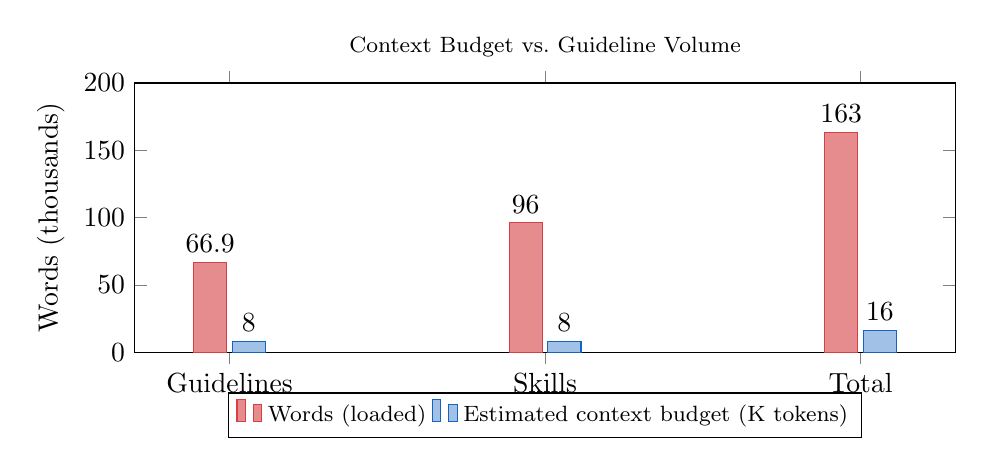
\begin{tikzpicture}
\begin{axis}[
  width=12cm, height=5cm,
  ybar,
  bar width=12pt,
  enlarge x limits=0.15,
  symbolic x coords={Guidelines,Skills,Total},
  xtick=data,
  nodes near coords,
  nodes near coords align={vertical},
  ylabel={Words (thousands)},
  ymin=0, ymax=200,
  title={Context Budget vs.\ Guideline Volume},
  title style={font=\footnotesize},
  legend style={at={(0.5,-0.15)}, anchor=north, legend columns=-1, font=\footnotesize}
]
\addplot[fill=accentred!60, draw=accentred] coordinates {(Guidelines,66.9) (Skills,96.0) (Total,163.0)};
\addplot[fill=accentblue!40, draw=accentblue] coordinates {(Guidelines,8) (Skills,8) (Total,16)};
\legend{Words (loaded), Estimated context budget (K tokens)}
\end{axis}
\end{tikzpicture}
\caption{The ratio of guideline/skill text volume (163K words) to typical context budget (16K token window).  Even with progressive disclosure, the orchestrator must hold the guidelines layer in context to enforce pipeline compliance.}
\label{fig:bloat}
\end{figure}

\subsection{Eight Specific Gaps}

\begin{gapbox}
\textbf{Gap 1: Trigger Keyword Ambiguity.}  Each SKILL.md declares \texttt{Triggers on:} keywords in its frontmatter (\S\ref{sec:triggers}).  These keywords are broad (e.g., ``approval, authorized, implement, start work, go ahead'' for approval-gate).  Multiple skills can match the same request.  Anthropic documented this failure mode: ``Claude Opus 4.5 and 4.6 has a strong predilection for subagents and may spawn them in situations where a simpler, direct approach would suffice.''\footnote{Anthropic.  ``Agent Skills Best Practices.''  \url{https://docs.anthropic.com/en/docs/agents-and-tools/agent-skills/best-practices}}  The escalation language in skills (``CRITICAL: You MUST use this tool when...'') accumulates model-specific assumptions that break when model capabilities change.

\textbf{Required fix:}  Trigger keywords should be \emph{disjoint} (no overlap between skills) or the routing resolution should be structural (first-match with precedence, not model-judgment).  The Agent Skills specification's progressive-disclosure model was designed for capabilities, not for workflow enforcement---using it for both creates ambiguity.

\textbf{Routing infrastructure note.}  The opencode CLI harness already injects a structured \texttt{<available\_skills>} block into the agent's system prompt containing each skill's name, description, and trigger keywords.\footnote{The \texttt{<available\_skills>} block is generated by the CLI harness from SKILL.md frontmatter at session start and injected into the system prompt before the first user message.  This pre-injection is a structural mechanism the agent does not see or reason about---it simply receives the block as part of its prompt.}  This pre-injection mechanism is the natural insertion point for structural routing: instead of relying on the agent to match trigger keywords against task descriptions, the harness could resolve skill selection at injection time---injecting only the skills whose pipeline-stage pre-conditions are satisfied.  This requires no changes to the agent's reasoning loop; it simply narrows what the agent sees.
\end{gapbox}

\begin{gapbox}
\textbf{Gap 2: Incomplete Clean-Room Enforcement.}  The clean-room dispatch protocol is specified (must-receive/must-not-receive context isolation in \texttt{divide-and-conquer/SKILL.md}) but there is \textbf{no audit trail} confirming that excluded context was actually excluded.  The orchestrator states ``I dispatched a clean-room sub-agent'' but there is no structural mechanism proving that the sub-agent did not receive implementation context, prior results, or cached verification.  This is the verification-equivalent of the ``metadata-as-evidence'' regression: the existence of a clean-room protocol is treated as evidence that clean-room dispatch occurred.

\textbf{Required fix:}  Sub-agent dispatch must include a \textbf{context hash} (checksum of the dispatch payload) that the orchestrator logs.  Post-dispatch verification compares the hash against known exclusions to confirm no excluded content was present.
\end{gapbox}

\begin{gapbox}
\textbf{Gap 3: Guideline Text Leaks Through Progressive Disclosure.}  Guidelines (26 files, 66,908 words) are loaded into the orchestrator's system prompt---they are \emph{not} lazily loaded.  This means every pipeline stage carries the full rulebook even when most rules never fire.  The ``lazy-loaded guidelines'' section in \texttt{060-tool-usage.md} mentions two files (065-verification-honesty.md, 067-context-completeness.md) but the remaining 24 guideline files lack a lazy-loading mechanism.

\textbf{Required fix:}  All guidelines should follow the progressive-disclosure model: each guideline file declares a trigger condition in frontmatter.  The orchestrator loads only the index (name + description pairs).  Full guideline text loads only when a verification gate fires.
\end{gapbox}

\begin{gapbox}
\textbf{Gap 4: Gap-Fill Cascade Can Skip Verification.}  When \texttt{authorization\_scope >= for\_plan}, missing artifacts are gap-filled automatically: spec missing $\to$ brainstorming creates it; plan missing $\to$ writing-plans creates it, etc.  This is correct for artifact \emph{existence} but can skip verification \emph{quality}.  A gap-filled spec created by the pipeline has no evidence artifacts attached to its acceptance criteria---the pipeline created the spec to satisfy a structural gate, not to verify claims.

\textbf{Required fix:}  Gap-filled artifacts must be annotated with a \texttt{GAP-FILLED} flag that triggers a deferred verification cycle.  Until verification passes, the gap-filled artifact is ``provisional'' and cannot be treated as authoritative at downstream gates.
\end{gapbox}

\begin{gapbox}
\textbf{Gap 5: No Structural Conflict Detection Between Skills.}  The deck has 45 skills with overlapping trigger keywords.  Nothing prevents two skills from both matching a request and producing conflicting instructions.  The agent resolves this through model judgment (``which skill seems more relevant?''), not through a structural conflict resolution mechanism.  Academic research on multi-agent hallucination specifically identifies ``conflicting instructions between skills'' as a failure mode.\footnote{Semantic Scholar taxonomy on multi-agent hallucination mitigation in coding agents.}

\textbf{Required fix:}  A skill-conflict resolver should run at dispatch time: detect overlapping trigger matches, compare must-receive/must-not-receive schemas, and resolve conflicts through precedence rules (not model reasoning).  Conflicting skill invocations should HALT and escalate, not proceed with the agent's guess.
\end{gapbox}

\begin{gapbox}
\textbf{Gap 6: Stale-Data Reliance Is a Guideline, Not a Structural Gate.}  The \texttt{065-verification-honesty.md} guideline is 425 lines of prose describing what constitutes evidence and what does not.  Despite this exhaustive specification, the agent \emph{still} relies on stale data because the enforcement mechanism is text-based: the agent reads the guideline and then decides (through chain-of-thought reasoning) whether its current claim needs verification.  This is the guardrail-bypass failure documented in the ``Governing What You Cannot Observe'' research: text guardrails can be rationalized away during chain-of-thought.

\textbf{Required fix:}  Stale-data prevention needs a \textbf{structural gate, not a text guideline.}  The session-enforcement.ts plugin could inject a context-age watermark before each agent turn: ``Last verification of [resource] at [timestamp].  Age: [seconds].  Threshold: [N seconds].''  The watermark is not text to be read and heeded---it is a structural signal that the agent's tool-call pipeline checks before accepting memory as evidence.
\end{gapbox}

\begin{gapbox}
\textbf{Gap 7: Preloaded Sub-Agent Context --- The Orchestrator Pollution Problem (NEW).}  Discovery from April 30--May 1 2026 investigation of concrete agent misbehavior.  Despite the clean-room dispatch protocol established in Gap~2, sub-agents still receive \emph{preloaded orchestrator reasoning} in their dispatch context.  The orchestrator performs analysis and design work inline, then hands sub-agents rote execution instructions (``edit file X at line 42 and replace A with B'').  The sub-agent is reduced to a file-editing command rather than an intelligent reasoning agent.

\textbf{This gap has three concrete manifestations:}

\begin{enumerate}[leftmargin=*]
  \item \textbf{Rote execution instructions.}  The orchestrator pre-determines exact file paths, line numbers, and replacement text.  The sub-agent executes the script without independently determining whether those are the correct changes.  Issue~\#273 is the canonical example: the orchestrator pre-determined 37 affected files but missed 44 files in \texttt{tools/} and \texttt{hooks/}.  If the sub-agent had been told \emph{what} to do (``replace all git rev-parse patterns with canonical walk-up'') rather than \emph{which files to edit}, it would have discovered the full scope by searching for the pattern independently.

  \item \textbf{Verification scope pollution.}  Verification sub-agents receive pre-selected file lists from the orchestrator.  They confirm what the orchestrator already believes---they never challenge scope, never discover missed changes, never flag adjacent breakage caused by the implementation.  The verifier cannot report on three critical questions: (a) were changes \emph{missed} that the spec required?  (b) did the change \emph{break} something in adjacent code?  (c) does a pre-existing bug discovered during verification need its own issue ticket?

  \item \textbf{The ``progressively reveal'' paradox.}  The orchestrator's ability to preload specific reasoning into sub-agents is enabled by the volume of knowledge loaded into its own context---67K words of guidelines and 96K words of SKILL.md bodies.  If the orchestrator only held a compact index (\textasciitilde{}2,500 words), it could not preload sub-agents with detailed file paths and expected outcomes.  The text bloat identified in Figure~\ref{fig:bloat} is not just a context-budget problem---it is the mechanism that enables all three sub-agent pollution patterns.

\end{enumerate}

\textbf{Required fix:}  Three structural changes, each tracked in its own issue:

\begin{enumerate}[leftmargin=*]
  \item [(i)] \textbf{Universal pre-analysis sub-agent gate} (spec \#274, \texttt{michael-conrad/.opencode}): every execution dispatch is preceded by an analysis sub-agent that receives only the spec/issue number and independently discovers scope, affected files, and returns a dispatch plan---the orchestrator routes based on the plan without semantic understanding of the work.
  \item [(ii)] \textbf{Autonomous verification deep-dive} (spec \#274): verification sub-agents receive success criteria only (no file lists, no scope restrictions) and independently search the codebase, triaging findings through a three-tier model (pre-existing bug $\to$ file issue ticket, regression caused by this change $\to$ remediate, fatal $\to$ abort).
  \item [(iii)] \textbf{Orchestrator context reduction} (spec \#276, \texttt{michael-conrad/.opencode}): progressive disclosure applied to all 26 guideline files (trigger frontmatter, index-only at startup at \textasciitilde{}1K words) and all 45 SKILL.md files (index-only, $\leq$600 words each, procedural workflow moved to task files).  Build-time \texttt{skildeck lint} rules enforce word-count limits and frontmatter presence.  Total orchestrator context $\leq$2,500 words.  Full procedural knowledge lives exclusively in ephemeral sub-agent windows.
\end{enumerate}
\end{gapbox}

\begin{gapbox}
\textbf{Gap 8: All Sub-Agents Are Identical \texttt{general} Agents --- No Role Taxonomy.}
The dispatch chain uses \texttt{task(subagent\_type="general")} for every
sub-agent regardless of its role in the pipeline.  The
\emph{implementation} sub-agent writing code, the \emph{verification}
sub-agent checking deliverables, and the \emph{audit} sub-agent reviewing
a spec all receive the same system prompt, the same 45-skill
\texttt{<available\_skills>} block with 258 overlapping trigger keywords,
and the same complete guideline set.  There is no structural difference
between a sub-agent dispatched to implement a spec and one dispatched
to verify the implementation.

\textbf{This gap amplifies every other gap.}  Trigger keyword ambiguity
(Gap~1) is a function of candidate-set size---an agent deliberating over
258 keywords across 45 skills has exponentially more bypass opportunities
than one deliberating over 24 keywords across 4 skills.  Clean-room
violations (Gaps~2,~7) are harder to prevent when the sub-agent carries
the full \texttt{approval-gate} and \texttt{divide-and-conquer} routing
logic in its context.  Stale-data rationalization (Gap~6) has more
guideline text to reason around.  Skill conflicts (Gap~5) have 990
possible cross-skill collision pairs.

\textbf{Required fix:} Named sub-agent role types with curated
skill-permission blocks in Markdown agent files
(\texttt{.opencode/agents/<role>.md}).  An \texttt{implementer} sees
\textasciitilde{}8 skills; a \texttt{verifier} sees \textasciitilde{}5
skills; a \texttt{pre-analyzer} sees \textasciitilde{}2 skills.  The
OpenCode platform's per-agent \texttt{permission.skill} configuration
supports this without new infrastructure---it requires only a taxonomy
of sub-agent roles and corresponding allowlist definitions.  Each role
carries a markdown file:

\begin{lstlisting}[style=pseudocode, language={}]
# .opencode/agents/verifier.md
---
description: Verifies implementation against spec success criteria
mode: subagent
permission:
  skill:
    "*": deny
    "verification-before-completion": allow
    "verification-enforcement": allow
    "verification": allow
    "issue-operations": allow
---
\end{lstlisting}

The orchestrator dispatches \texttt{task(subagent\_type="verifier")}
instead of \texttt{task(subagent\_type="general")}.  The verifier's
\texttt{<available\_skills>} block contains 4 descriptor entries
(\textasciitilde{}120 words) instead of 45 (\textasciitilde{}1,350
words).  Trigger-keyword overlap is reduced 10.7$\times$---from 258
candidate keywords to 24.  Cross-role skill conflicts become structurally
impossible: a verifier cannot invoke \texttt{divide-and-conquer} or
\texttt{writing-plans} because those skills are not in its allowlist.
The Single Concern Principle moves from a text-based guideline to a
runtime constraint.
\end{gapbox}

\newpage

%=====================================================================
\section{The Unix-Philosophy-Aligned Skill Deck}

\subsection{Core Principles Applied}

What would a skill deck look like that fully embraces the Unix philosophy?  Table~\ref{tab:rethink} re-architects each deck component.

\begin{table}[htbp]
\centering
\caption{Unix-Aligned Re-Architecture}
\label{tab:rethink}
\small
\begin{tabular}{@{}p{3cm}p{4.2cm}p{5.5cm}@{}}
\toprule
\textbf{Component}      & \textbf{Current State}                    & \textbf{Unix-Aligned State} \\
\midrule
Guidelines              & 26 files, 67K words, loaded at startup    & 26 files with progressive-disclosure frontmatter.  Index only (name + trigger-pattern) loaded at startup (\textasciitilde{}1K words).  Full body lazy-loaded on gate activation. \\
\midrule
Skills (SKILL.md)       & 45 files, 96K words; trigger keywords ambiguous; escalation language embedded & 45 files with disjoint trigger patterns; no escalation language (``CRITICAL:'' $\to$ structural flag); each $\leq$600 words (Unix: ``do one thing well'').  Execution moved to task files. \\
\midrule
Task files              & 237 files, many exceeding 3K-word limit   & 237 files, each $\leq$3K words enforced at build time.  Each task is a single-purpose sub-agent dispatch instruction.  Output format specified as structured contract. \\
\midrule
Dispatch chain          & Hardcoded sequential pipeline              & DAG-based composition: stages declare input/output contracts.  Pipeline assembled at dispatch time from contract compatibility. \\
\midrule
Result contracts        & Specified per-skill, not universally enforced & Universal schema: \texttt{\{status, files, summary, evidence\_artifacts\}}.  Contract validator runs as a structural gate before orchestrator accepts output. \\
\midrule
Verification gates      & Text-based guideline enforcement           & Structural watermarks injected by session-enforcement plugin.  Context-age timestamp before each turn.  Claims without corresponding tool call in the age window are rejected. \\
\midrule
Sub-agent dispatch      & Clean-room protocol specified but not audited & Dispatch context hash logged.  Post-dispatch hash comparison confirms exclusions.  \texttt{must-not-receive} violations flagged as STRUCTURE-VIOLATION. \\
\midrule
Trigger routing         & Model-judgment based on keyword overlap    & Disjoint trigger patterns per skill.  Conflict resolver runs at dispatch: overlapping matches $\to$ precedence rules, not model guess.  Unresolvable conflicts $\to$ HALT + escalate. \\
\midrule
Skill invocation        & Agent decides which skill to invoke        & Pipeline stages declare required skills.  Missing invocation $\to$ pipeline HALT (not post-hoc detection). \\
\midrule
Gap-filled artifacts    & Treated as authoritative immediately       & Flagged \texttt{GAP-FILLED} + deferred verification cycle.  Cannot pass downstream gates until evidence artifacts exist. \\
\midrule
Sub-agent types        & 1 type (\texttt{general}) used for all dispatches.  All 45 skills visible to every sub-agent. 258 overlapping trigger keywords. & 12+ named role types defined as \texttt{.opencode/agents/<role>.md} markdown files: \texttt{spec-explorer}, \texttt{plan-writer}, \texttt{pre-worker}, \texttt{pre-analyzer}, \texttt{implementer}, \texttt{verifier}, \texttt{auditor}, \texttt{pr-creator}, \texttt{correspondent}, \texttt{runbooker}, \texttt{debugger}, \texttt{reviewer}, \texttt{ui-builder}, \texttt{skill-builder}.  Each has curated \texttt{permission.skill} allowlist (3--8 skills).  Trigger-keyword overlap reduced 4$\times$--43$\times$ per agent.  Cross-role skill conflicts structurally impossible. \\
\bottomrule
\end{tabular}
\end{table}

\subsection{Clean-Room Dispatch Protocol (Complete)}

Figure~\ref{fig:cleanroom} shows the complete clean-room dispatch protocol, including the context-hash audit trail that the current deck lacks.

\begin{figure}[htbp]
\centering
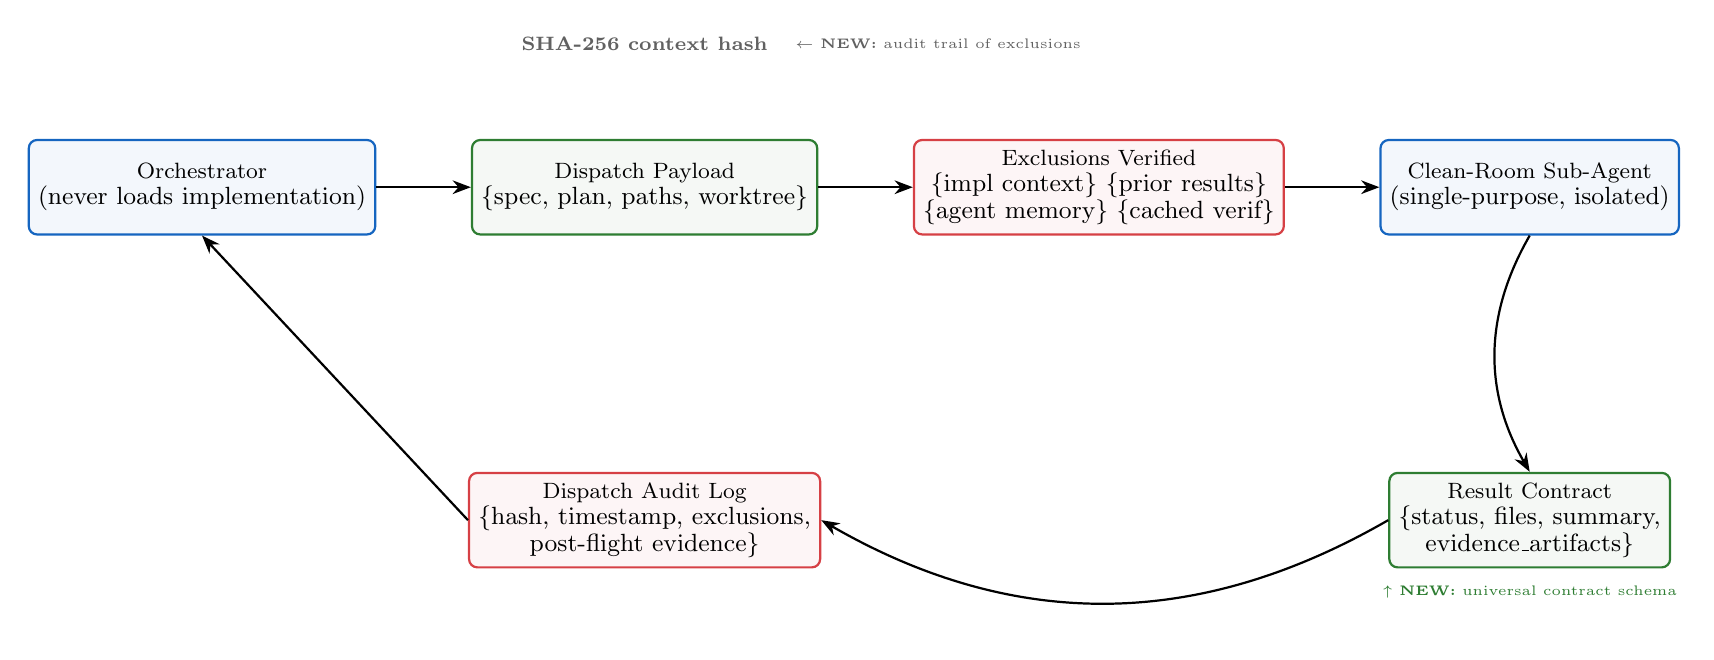
\begin{tikzpicture}[
  node distance=10mm and 12mm,
  obox/.style={
    draw=accentblue, rounded corners=3pt, minimum width=3.3cm, minimum height=1.2cm,
    align=center, font=\footnotesize, fill=accentblue!5, thick,
  },
  rbox/.style={
    draw=accentgreen, rounded corners=3pt, minimum width=3.3cm, minimum height=1.2cm,
    align=center, font=\footnotesize, fill=accentgreen!5, thick,
  },
  ebox/.style={
    draw=accentred, rounded corners=3pt, minimum width=3.3cm, minimum height=1.2cm,
    align=center, font=\footnotesize, fill=accentred!5, thick,
  },
  arrow/.style={->, >=Stealth, thick},
  label/.style={font=\scriptsize\bfseries, text=accentgray},
]

\node[obox] (orchestrator) {Orchestrator\\\small(never loads implementation)};

\node[rbox, right=of orchestrator] (dispatch) {Dispatch Payload\\\small\{spec, plan, paths, worktree\}};

\node[label, above=of dispatch] (hashlabel) {SHA-256 context hash};

\node[ebox, right=of dispatch] (exclusions) {Exclusions Verified\\\small\{impl context\} \{prior results\}\\\small\{agent memory\} \{cached verif\}};

\node[obox, right=of exclusions] (subagent) {Clean-Room Sub-Agent\\\small(single-purpose, isolated)};

\node[rbox, below=3cm of subagent] (result) {Result Contract\\\small\{status, files, summary,\\\small evidence\_artifacts\}};

\node[ebox, below=3cm of dispatch] (audit) {Dispatch Audit Log\\\small\{hash, timestamp, exclusions,\\\small post-flight evidence\}};

% arrows
\draw[arrow] (orchestrator) -- (dispatch);
\draw[arrow] (dispatch) -- (exclusions);
\draw[arrow] (exclusions) -- (subagent);
\draw[arrow, bend right=30] (subagent.south) to (result.north);
\draw[arrow, bend left=30] (result.west) to (audit.east);
\draw[arrow] (audit.west) -- (orchestrator.south);

% annotations
\node[font=\tiny, text=accentgray, right=0.1cm of hashlabel.east, anchor=west] {$\leftarrow$ \textbf{NEW:} audit trail of exclusions};
\node[font=\tiny, text=accentgreen, below=0.1cm of result.south, anchor=north] {$\uparrow$ \textbf{NEW:} universal contract schema};

\end{tikzpicture}
\caption{Complete clean-room dispatch with context-hash audit trail.  The two elements marked \textbf{NEW} are the structural additions that the current deck lacks---without them, clean-room dispatch is a protocol description, not an enforced invariant.}
\label{fig:cleanroom}
\end{figure}

\subsection{Trigger Semantics (Disjoint)}

Figure~\ref{fig:triggers} illustrates the difference between the current overlapping trigger model and the proposed disjoint trigger model.

\begin{figure}[htbp]
\centering
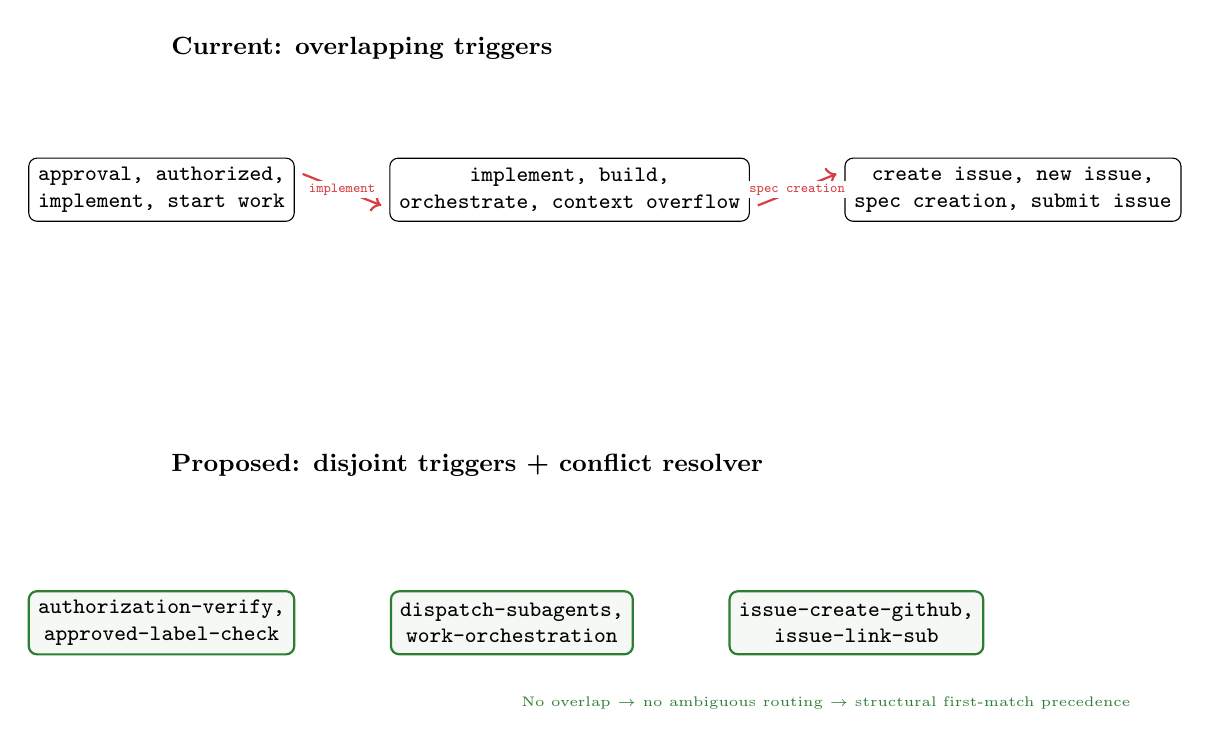
\begin{tikzpicture}[
  node distance=8mm and 12mm,
  skillB/.style={
    draw, rounded corners=3pt, minimum width=2.4cm, minimum height=0.8cm,
    align=center, font=\footnotesize\ttfamily, fill=white,
  },
  overlap/.style={
    draw=accentred, rounded corners=3pt, minimum width=1.5cm, minimum height=0.8cm,
    align=center, font=\tiny, fill=accentred!10, thick,
  },
  disjoint/.style={
    draw=accentgreen, rounded corners=3pt, minimum width=2.4cm, minimum height=0.8cm,
    align=center, font=\footnotesize\ttfamily, fill=accentgreen!5, thick,
  },
]

% Current state label
\node[font=\small\bfseries, anchor=west] at (0,1.8) {Current: overlapping triggers};
\node[skillB] (s1) at (0,0) {approval, authorized,\\implement, start work};
\node[skillB, right=of s1] (s2) {implement, build,\\orchestrate, context overflow};
\node[skillB, right=of s2] (s3) {create issue, new issue,\\spec creation, submit issue};

\draw[accentred, thick, ->] ($(s1.east)+(0.1,0.2)$) -- ($(s2.west)-(0.1,0.2)$)
  node[midway, font=\tiny, fill=white, inner sep=1pt] {\texttt{implement}};
\draw[accentred, thick, ->] ($(s2.east)+(0.1,-0.2)$) -- ($(s3.west)-(0.1,-0.2)$)
  node[midway, font=\tiny, fill=white, inner sep=1pt] {\texttt{spec creation}};

% Proposed state label
\node[font=\small\bfseries, anchor=west] at (0,-3.5) {Proposed: disjoint triggers + conflict resolver};
\node[disjoint] (d1) at (0,-5.5) {authorization-verify,\\approved-label-check};
\node[disjoint, right=of d1] (d2) {dispatch-subagents,\\work-orchestration};
\node[disjoint, right=of d2] (d3) {issue-create-github,\\issue-link-sub};

\node[font=\tiny, text=accentgreen, anchor=west] at ($(d2.south)+(0,-0.6)$) {No overlap $\to$ no ambiguous routing $\to$ structural first-match precedence};

\end{tikzpicture}
\caption{Overlapping triggers (top) create routing ambiguity resolved by model judgment.  Disjoint triggers (bottom) with a structural conflict resolver eliminate ambiguity---if two skills match, the conflict resolver applies precedence rules, not the agent's guess.}
\label{fig:triggers}
\end{figure}

\newpage

%=====================================================================
\section{The Unix Pipeline Model for Sub-Agents}

\subsection{Why Scope-Limited Single-Purpose Sub-Agents}

The Unix philosophy's insight about composing small programs through pipes maps directly to sub-agent decomposition~\cite{piskala2026unix}.  The research validates this:

\begin{enumerate}[leftmargin=*]
  \item \textbf{GraSP (Xia et al.)} found that DAG-based skill composition with precondition-effect edges outperforms flat invocation in every configuration (+19 reward points, -41\% environment steps).\footnote{Xia et al.  ``GraSP: Graph-Structured Skill Compositions for LLM Agents.''  arXiv:2604.17870, April 2026.}
  \item \textbf{AgentSpawn (Costa)} showed that dynamic spawning with automatic memory transfer achieves 34\% higher completion than static baselines.
  \item \textbf{SkillCraft (Chen et al.)} demonstrated that token usage drops by up to 80\% through skill caching and reuse.
  \item \textbf{Debug2Fix (Garg \& Huang)} proved that ``better tool design is often just as important as switching to a more expensive model''---weaker models match stronger models through architecture alone.
\end{enumerate}

The current deck's fixed dispatch chain is correct in principle but \textbf{too rigid.}  A Unix pipeline is compositional: each stage does one thing, and stages can be recombined in different orders for different workflows.  The current deck hardcodes the pipeline---all authorized work flows through the same sequence regardless of what the work actually needs.

\subsection{Proposed: Contract-Based Pipeline Assembly}

\begin{insightbox}
\textbf{Contract-based composition.}  Each pipeline stage declares (a) its input contract (what data it expects), (b) its output contract (what data it produces), and (c) its exclusions (what must NOT be in context).  The pipeline assembler reads the spec's requirements and selects stages whose contracts satisfy the requirements.  This is \emph{compose(1)} for agent workflows.
\end{insightbox}

\begin{figure}[htbp]
\centering
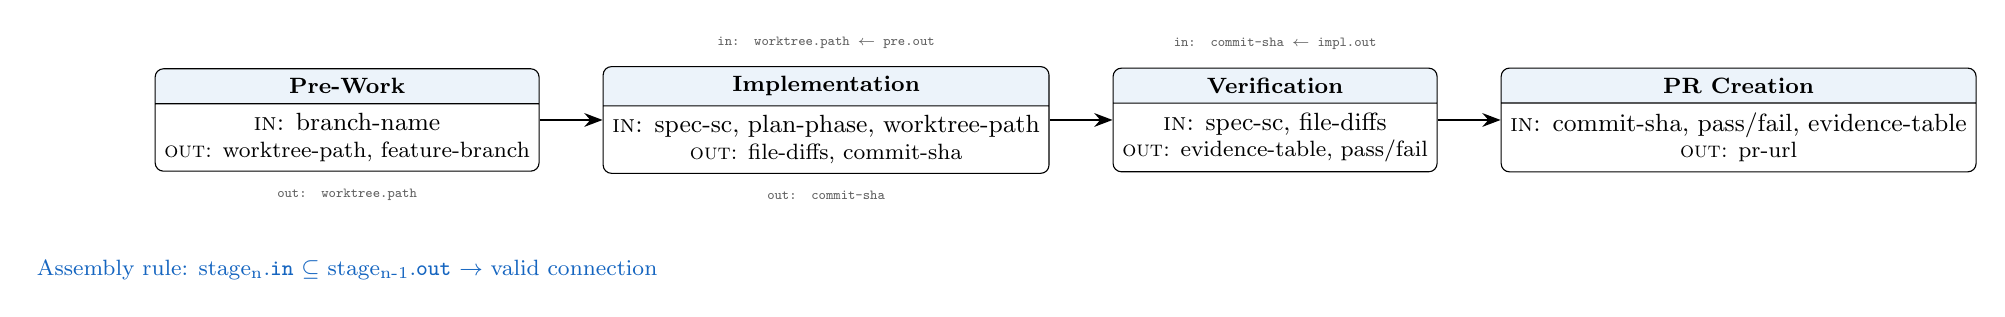
\begin{tikzpicture}[
  node distance=7mm and 8mm,
  stage/.style={
    draw, rectangle split, rectangle split parts=2,
    rectangle split part fill={accentblue!8,white},
    minimum width=3.8cm, minimum height=1.4cm,
    align=center, font=\footnotesize, rounded corners=3pt,
  },
  arrow/.style={->, >=Stealth, thick},
  contract/.style={font=\tiny\ttfamily, text=accentgray},
]

\node[stage] (pre) {
  \nodepart{one} \textbf{Pre-Work}
  \nodepart{two} \small\textsc{in:} branch-name\\
                  \textsc{out:} worktree-path, feature-branch
};

\node[stage, right=of pre] (impl) {
  \nodepart{one} \textbf{Implementation}
  \nodepart{two} \small\textsc{in:} spec-sc, plan-phase, worktree-path\\
                  \textsc{out:} file-diffs, commit-sha
};

\node[stage, right=of impl] (verify) {
  \nodepart{one} \textbf{Verification}
  \nodepart{two} \small\textsc{in:} spec-sc, file-diffs\\
                  \textsc{out:} evidence-table, pass/fail
};

\node[stage, right=of verify] (pr) {
  \nodepart{one} \textbf{PR Creation}
  \nodepart{two} \small\textsc{in:} commit-sha, pass/fail, evidence-table\\
                  \textsc{out:} pr-url
};

\draw[arrow] (pre) -- (impl);
\draw[arrow] (impl) -- (verify);
\draw[arrow] (verify) -- (pr);

% Contract flow annotations
\node[contract, below=0.1cm of pre] {\texttt{out: worktree.path}};
\node[contract, above=0.1cm of impl] {\texttt{in: worktree.path $\leftarrow$ pre.out}};
\node[contract, below=0.1cm of impl] {\texttt{out: commit-sha}};
\node[contract, above=0.1cm of verify] {\texttt{in: commit-sha $\leftarrow$ impl.out}};

% Assembly note
\node[font=\footnotesize, text=accentblue, anchor=north, below=1cm of pre] {
  Assembly rule: stage\textsubscript{n}.\texttt{in} $\subseteq$ stage\textsubscript{n-1}.\texttt{out}  $\to$  valid connection
};

\end{tikzpicture}
\caption{Contract-based pipeline assembly.  Stages declare input/output contracts.  The assembler connects stages whose contracts are compatible.  This replaces the current hardcoded dispatch chain with composable Unix-style pipes.}
\label{fig:contracts}
\end{figure}

\newpage

%=====================================================================
\section{Trigger Semantics and Structural Routing}
\label{sec:triggers}

\subsection{The Current Model: Description-Based Discovery}

The Agent Skills specification uses a description-based discovery model: agents load skill \texttt{name} + \texttt{description} pairs and route to a skill when its description matches the current task.  The current deck extends this by also listing explicit trigger keywords in each SKILL.md frontmatter.

This model works for \emph{capabilities} (``skill that extracts text from PDFs'') because the agent can reason about whether a PDF-extraction capability is relevant to the task.  It breaks down for \emph{workflow enforcement} (``skill that MUST run before any implementation'') because:

\begin{enumerate}[leftmargin=*]
  \item The agent must \emph{detect} that it is in an implementation workflow (judgment call)
  \item The agent must \emph{select} the correct enforcement skill from potentially overlapping candidates (judgment call)
  \item The agent must \emph{decide} whether to invoke the skill now or later (judgment call)
\end{enumerate}

Each of these judgment calls is a point where the agent can rationalize a shortcut.  The research on agent failure modes confirms that these judgment points are exactly where guardrail bypass occurs.\footnote{``Governing What You Cannot Observe: Adaptive Runtime Governance for Autonomous AI Agents.''  Semantic Scholar.}

\subsection{Proposed: Pipeline-Stage Declarations}

Instead of trigger keywords that the agent matches against task descriptions, each pipeline stage should \textbf{declare required skills} as pre-conditions.  The orchestrator checks pre-conditions, not the agent:

\begin{lstlisting}[style=pseudocode, language={}]
# Current: agent matches trigger keywords against task description
Skill: approval-gate
Triggers on: approval, authorized, implement, start work, go ahead

# Proposed: pipeline stage declares required skills as pre-conditions
Stage: verify-authorization
Requires: [approval-gate/verify-authorization]
Pre-conditions:
  - auth_phrase_parsed == true
  - scope_resolved == true
  - halt_at_set == true
Output-contract: {status, scope, halt_at, pr_strategy, issues[]}

Stage: pre-work
Requires: [git-workflow/pre-work]
Pre-conditions:
  - Previous stage completed with status: PASS
  - worktree.path is NOT set (pre-work creates it)
Output-contract: {worktree.path, feature-branch, commit-hash, push-status}

Stage: implementation
Requires: [divide-and-conquer/assemble-work]
Sub-agent-type: implementer
Permission:
  skill.deny: ["*"]
  skill.allow: [test-driven-development, code-size-enforcement,
                engineering-approach, programming-principles,
                mcp-tool-usage, notebook-operations, issue-operations]
Pre-conditions:
  - spec approved (verified via approved-for-* label)
  - plan with valid sub-issue structure exists
  - worktree.path is set
Exclusions:
  - Verification success criteria (must-not-receive)
  - Audit findings from prior work
Output-contract: {status, files_changed, commit-sha, per-sc-traceability}

Stage: verification
Requires: [verification-before-completion/verify]
Sub-agent-type: verifier
Permission:
  skill.deny: ["*"]
  skill.allow: [verification-before-completion, verification-enforcement,
                verification, issue-operations]
Pre-conditions:
  - implementation commit exists (verified via git log)
  - all implementation sub-agents returned DONE or DONE_WITH_CONCERNS
Exclusions:
  - Implementation source code (must-not-receive)
  - Prior verification results from other phases
  - Agent memory from implementation sub-agents
Output-contract: {status, evidence-table, per-sc-pass-fail, concerns[]}
\end{lstlisting}

\begin{insightbox}
\textbf{Why this works.}  The orchestrator loads the pipeline definition (a list of stages with required skills and pre-conditions).  It checks pre-conditions mechanically (``did the previous stage return \texttt{status: PASS}?''), not semantically (``does the previous stage seem like it completed correctly?'').  Mechanical checks are deterministic; semantic checks are rationalizable.  This is the same difference as between a file-existence check and a code-review judgment.
\end{insightbox}

\newpage

%=====================================================================
\section{Implementation Complexity Audit}

\subsection{Skill File Size Analysis}

The ``do one thing well'' principle requires that each skill be small enough to load without context degradation and focused enough that its trigger is unambiguous.  Table~\ref{tab:complexity} shows the most complex skills by file count and estimated context budget.

\begin{table}[htbp]
\centering
\caption{Top Skills by Complexity}
\label{tab:complexity}
\small
\begin{tabular}{@{}p{3.8cm}rrp{3cm}@{}}
\toprule
\textbf{Skill}              & \textbf{SKILL.md Words} & \textbf{Associated Tasks} & \textbf{Roles Where Visible} \\
\midrule
approval-gate               & $>$3,500 (est.)         & 16 task files             & orchestrator only \\
git-workflow                & $>$3,000 (est.)         & 12+ task files            & orchestrator, pre-worker, pr-creator \\
divide-and-conquer          & $>$2,500 (est.)         & 8 task files              & orchestrator only \\
verification-before-completion & $>$2,000 (est.)      & 6 task files              & orchestrator, verifier \\
issue-operations            & $>$2,500 (est.)         & 10+ task files            & universal (all roles) \\
\bottomrule
\end{tabular}
\end{table}

\begin{gapbox}
\textbf{The anti-Unix pattern.}  When a skill's SKILL.md exceeds the 3,000-word atomicity threshold (the rule applied to task files), the skill itself violates the ``do one thing well'' principle.  The orchestrator loads SKILL.md to route to the correct task, but SKILL.md has grown to include routing logic, dispatch schemas, pre/post-conditions, audit tables, cross-references, completion guarantees, and worktree-mode instructions---all in a single file.  This is the equivalent of a Unix program whose man page is longer than its executable.

\textbf{Required fix:}  SKILL.md files should be \textbf{index files only}: name, description, trigger pattern (disjoint), and a list of task references with their input/output contracts.  The task files contain the procedural workflow.  The orchestrator reads the index (compact), dispatches to the correct task sub-agent (which loads the task file in its own context window), and receives a result contract.  No SKILL.md should exceed 600 words.
\end{gapbox}

\subsection{The Guideline Loading Problem}

Figure~\ref{fig:loading} illustrates the current guideline loading model vs.\ the proposed progressive-disclosure model.

\begin{figure}[htbp]
\centering
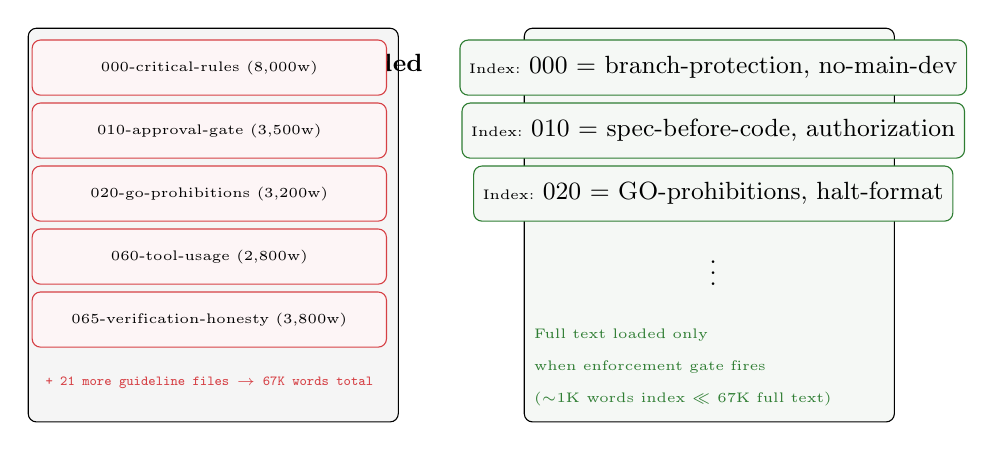
\begin{tikzpicture}[
  node distance=6mm and 8mm,
  bigB/.style={
    draw=accentred, rounded corners=3pt, minimum width=4.5cm, minimum height=0.7cm,
    align=center, font=\tiny, fill=accentred!5,
  },
  smallB/.style={
    draw=accentgreen, rounded corners=3pt, minimum width=4.5cm, minimum height=0.7cm,
    align=center, font=\tiny, fill=accentgreen!5,
  },
]

% Left side - Current
\draw[fill=bglight, rounded corners=3pt] (-5.5,0.5) rectangle (-0.8,-4.5);
\node[font=\small\bfseries, anchor=north west] at (-5.5,0.3) {Current: all guidelines loaded};

\node[bigB] (g1) at (-3.2, 0.0) {000-critical-rules (8,000w)};
\node[bigB] (g2) at (-3.2,-0.8) {010-approval-gate (3,500w)};
\node[bigB] (g3) at (-3.2,-1.6) {020-go-prohibitions (3,200w)};
\node[bigB] (g4) at (-3.2,-2.4) {060-tool-usage (2,800w)};
\node[bigB] (g5) at (-3.2,-3.2) {065-verification-honesty (3,800w)};
\node[font=\tiny\ttfamily, text=accentred] at (-3.2,-4.0) {+ 21 more guideline files $\to$ 67K words total};

% Right side - Proposed
\draw[fill=accentgreen!5, rounded corners=3pt] (0.8,0.5) rectangle (5.5,-4.5);
\node[font=\small\bfseries, anchor=north west] at (0.8,0.3) {Proposed: progressive disclosure};

\node[smallB] (p1) at (3.2, 0.0) {Index: {\small 000 = branch-protection, no-main-dev}};
\node[smallB] (p2) at (3.2,-0.8) {Index: {\small 010 = spec-before-code, authorization}};
\node[smallB] (p3) at (3.2,-1.6) {Index: {\small 020 = GO-prohibitions, halt-format}};
\node[font=\small] at (3.2,-2.5) {$\vdots$};

\node[font=\tiny, text=accentgreen, anchor=north west] at (0.8,-3.2) {Full text loaded only};
\node[font=\tiny, text=accentgreen, anchor=north west] at (0.8,-3.6) {when enforcement gate fires};
\node[font=\tiny, text=accentgreen, anchor=north west] at (0.8,-4.0) {($\sim$1K words index $\ll$ 67K full text)};

\end{tikzpicture}
\caption{Left: current model loads all guideline text into the orchestrator's context ($\sim$67K words).  Right: progressive-disclosure model loads only name + trigger-pattern index ($\sim$1K words), loading full text when an enforcement gate fires.  This maps to the ``do one thing well'' principle: each guideline file is a single rule, loaded only when relevant.}
\label{fig:loading}
\end{figure}

\newpage

%=====================================================================
\section{Recommendations: From Text-Based to Structural Enforcement}

\subsection{The Six Shifts}
\label{sec:shifts}

The deck's core problem is that its enforcement mechanisms are \textbf{text-based rules} that the agent must read, understand, and voluntarily comply with.  The research shows that text-based enforcement fails because agents rationalize shortcuts during chain-of-thought reasoning.  The fix is to move from text-based to structural enforcement.  Table~\ref{tab:shifts} defines six concrete shifts.

\begin{table}[htbp]
\centering
\caption{Six Shifts: Text-Based $\to$ Structural Enforcement}
\label{tab:shifts}
\small
\begin{tabular}{@{}p{3.2cm}p{4.3cm}p{5cm}@{}}
\toprule
\textbf{Enforcement Domain} & \textbf{Current: Text-Based}             & \textbf{Proposed: Structural} \\
\midrule
1. Skill routing
  & Agent reads \texttt{Triggers on:} keywords and decides which skill to invoke
  & Pipeline stage declares \texttt{Requires:} skill list.  Orchestrator checks mechanically.  Missing $\to$ HALT \\
\midrule
2. Clean-room isolation
  & Agent reads dispatch context schema and voluntarily excludes
  & Context hash logged.  Post-dispatch hash comparison confirms \texttt{must-not-receive} exclusions.  Violation $\to$ BLOCKED \\
\midrule
3. Stale-data prevention
  & Agent reads 065-verification-honesty guideline and decides whether to verify
  & Session-enforcement injects context-age watermark before each turn.  Claims without tool call within age window $\to$ rejected \\
\midrule
4. Guideline compliance
  & All 26 guideline files loaded into context; agent applies relevant ones
  & Progressive disclosure: index only loaded.  Full guideline text loaded when enforcement gate fires.  Gate declares which guideline it enforces \\
\midrule
5. Verification evidence
  & Agent reads verification-enforcement SKILL.md and collects evidence voluntarily
  & Result contract validator: output without evidence artifacts $\to$ REJECT + RE-DISPATCH.  Contract schema enforced at pipeline boundary \\
\midrule
6. Sub-agent role taxonomy
  & Agent dispatches as generic \texttt{general} type; all 45 skills visible regardless of role; 258 candidate keywords to deliberate over
  & Named agent types (\texttt{implementer}, \texttt{verifier}, \texttt{pre-analyzer}, \texttt{auditor}, etc.) defined as \texttt{.opencode/agents/<role>.md} markdown files.  Each type has curated \texttt{permission.skill} allowlist (3--8 skills).  Role-inappropriate skills structurally invisible---\texttt{<available\_skills>} block shrinks from \textasciitilde{}1,350 words to \textasciitilde{}120--210 words.  Trigger-keyword overlap reduced 4$\times$--43$\times$ per agent.  Cross-role skill conflicts impossible by construction. \\
\bottomrule
\end{tabular}
\end{table}

\subsection{Priority Ordering}
\label{sec:priority}

The gaps identified in \S\ref{sec:gaps} have different severity levels.  Table~\ref{tab:priority} orders them by impact on the primary failure modes (skill confusion, stale-data reliance, premature completion).

\begin{insightbox}
\textbf{Alignment with existing tracking.}  The remediation priorities above are not proposed in a vacuum.  Issue \#248 (Gate Dependency Tree --- Prescriptive Runtime Enforcement Pipeline) already tracks a 5-gate progression from dispatch-entry pre-commit hooks through orchestrator-purity enforcement to per-SC evidence gates.  The paper's recommendations augment this existing pipeline rather than creating a parallel one: the context-age watermark (shift~3) plugs into Gate~1.5 (PR API Intercept), the context-hash audit trail (shift~2) strengthens Gate~3 (Orchestrator Purity), and progressive guideline disclosure (shift~4) reduces the text volume that Gate~2 (Dispatch Temporal Bound) must manage.  The remediation steps described in the next section map each shift onto an existing gate in \#248's dependency tree.
\end{insightbox}

\subsection{Tension: Structural Routing vs.\ Agent-Driven Discovery}

The paper recommends structural routing---fixed pipeline-stage declarations with mechanical pre-condition checks.  Two existing open issues propose complementary or partially conflicting approaches:

\begin{enumerate}[leftmargin=*]
  \item \textbf{Issue \#80} proposes \emph{agent-driven issue graph discovery} for the cleanup workflow, replacing static keyword parsing with LLM-inferred relationships.  This is correct for \textbf{open-ended graph traversal} where the number of connected issues cannot be predicted and relationship patterns are unbounded.  The paper's structural routing does \emph{not} apply here---graph discovery is a genuinely agentic task that benefits from LLM reasoning.
  \item \textbf{Issue \#179} argues for \textbf{prose over static templates}, warning that rigid structural formats produce mechanical compliance rather than genuine understanding.  This is a legitimate concern.  The paper's ``structural enforcement'' is \emph{not} template rigidity---it is runtime checking by code rather than the agent reading prose and deciding.  A structural gate does not say ``the spec must have exactly 5 sections'' (template); it says ``the spec must have tool-call evidence for each acceptance criterion claim'' (runtime check).  The former is template bureaucracy; the latter is enforcement.  The paper recommends the latter.
\end{enumerate}

\begin{insightbox}
\textbf{Resolution principle.}  Structural routing applies where the pipeline is \textbf{fixed}---every authorization follows the same stages, every stage has known pre-conditions, and the orchestrator's routing decisions are mechanical.  Agent-driven discovery applies where the pipeline is \textbf{open}---issue graph traversal, relationship inference, and completeness judgment require semantic reasoning that static patterns cannot encode.  The deck needs both, but it must distinguish them by pipeline stage: stages with fixed pre-conditions use structural routing; stages with unbounded discovery use agent-driven search.  Confusing them---applying structural routing to graph discovery or agent-driven search to dispatch-chain enforcement---is the anti-pattern to avoid.
\end{insightbox}

\begin{table}[htbp]
\centering
\caption{Gap Remediation Priority}
\label{tab:priority}
\small
\begin{tabular}{@{}clp{4cm}p{5cm}@{}}
\toprule
\textbf{Priority} & \textbf{Gap} & \textbf{Impact if Unfixed} & \textbf{Remediation} \\
\midrule
\textbf{P0} & Preloaded sub-agent context (Gap 7, NEW) & Orchestrator preloads rote file/line instructions into sub-agents.  Sub-agents reduced to file-editing commands; clean-room isolation bypassed.  Evidence: \#273 missed 44 files. & Universal pre-analysis sub-agent gate + autonomous verification deep-dive + orchestrator context reduction to index-only ($\leq$2,500 words).  Tracked in spec \#274. \\
\midrule
\textbf{P0} & Guideline bloat & Agent spends context budget reading rules instead of executing work.  The 163K-word rulebook defeats its own purpose. & Progressive disclosure for all 26 guideline files.  Index only ($\sim$1K words) loaded at startup. \\
\midrule
\textbf{P0} & No clean-room audit trail & Agent can claim clean-room dispatch without evidence.  Same class as \#91 (metadata-as-evidence). & Context-hash logging + post-dispatch hash comparison.  Violations flagged as STRUCTURE-VIOLATION. \\
\midrule
\textbf{P1} & Trigger keyword ambiguity & Multiple skills match same request.  Agent resolves through model judgment---the same judgment that rationalizes shortcuts. & Disjoint trigger patterns.  Conflict resolver with precedence rules.  Unresolvable $\to$ HALT. \\
\midrule
\textbf{P1} & Text-based stale-data enforcement & Agent reads the rule and decides whether to follow it.  Rule text cannot prevent rationalization. & Context-age watermark injected structurally by session-enforcement plugin.  Checked before claims are accepted. \\
\midrule
\textbf{P1} & Gap-fill cascade skips verification & Pipeline creates artifacts to satisfy structural gates but evidence artifacts are missing.  Artifacts treated as authoritative. & GAP-FILLED flag + deferred verification cycle.  Artifacts are provisional until evidence exists. \\
\midrule
\textbf{P2} & No skill conflict detection & 45 skills with overlapping triggers.  Nothing prevents conflicting invocations. & Conflict resolver at dispatch time.  Overlapping matches $\to$ precedence, not model judgment. \\
\midrule
\textbf{P2} & SKILL.md exceeds atomicity threshold & Skills violate their own 3,000-word rule.  Orchestrator loads verbose routing logic in its own context. & SKILL.md as index-only: name + description + trigger + task references.  $\leq$600 words each. \\
\midrule
\textbf{P2} & Fixed pipeline rigidity & All authorized work follows the same hardcoded chain regardless of what the work needs. & Contract-based pipeline assembly.  Stages declare input/output contracts.  Assembler selects stages. \\
\midrule
\textbf{P2} & Identical sub-agent types (Gap 8) & Every sub-agent sees 45 skills and 258 keywords regardless of role.  Amplifies Gaps 1, 2, 5, 6, and 7. & Named agent types (\texttt{.opencode/agents/<role>.md}) with curated \texttt{permission.skill} allowlists.  4$\times$--43$\times$ reduction in candidate skills per agent. \\
\bottomrule
\end{tabular}
\end{table}

\newpage

%=====================================================================
\section{Conclusion}

The opencode-config skill deck represents the most architecturally ambitious agent governance system we have encountered.  Its five core innovations---pure orchestrator, pipeline-scoped authorization, tiered mandates, tool-call evidence requirements, and plan-bridge hierarchy---are validated by the emerging academic literature and have no equivalent in any surveyed system.  The Unix philosophy of ``do one thing well'' is precisely the design framework that the deck \emph{aspires} to implement~\cite{piskala2026unix}.

The gap is not in aspiration but in implementation.  The deck enforces its protocols through \textbf{text-based rules} that the agent loads, reads, and voluntarily complies with.  Text-based enforcement is rationalizable: the agent can read a rule, decide (during chain-of-thought reasoning) that it does not apply in this specific case, and proceed with the shortcut.  The academic literature confirms that this is the primary failure mode for autonomous agent systems.

The Unix philosophy solves this problem by making enforcement \textbf{structural, not textual}.  A Unix pipe does not ``read a guideline about how to compose programs''---the pipe \emph{is} the composition mechanism.  The skill deck needs the same shift:

\begin{itemize}[leftmargin=*]
  \item Trigger routing should be a structural conflict resolver, not a model judgment about keyword relevance.
  \item Clean-room dispatch should be a context-hash audit trail, not a prose description of exclusion categories.
  \item Stale-data prevention should be a timestamp watermark injected by the runtime, not a guideline that the agent reads and heeds.
  \item Guideline loading should follow progressive disclosure (index only at startup), not eager loading of 67K words into the orchestrator's context.
  \item Skill metadata should be compact index files ($\leq$600 words), not verbose documents that exceed the deck's own atomicity threshold.
\end{itemize}

The research supports the deck's direction.  GraSP, CAID, NeuroClaw, Debug2Fix, and Anthropic's own engineering essays all converge on structured pipeline orchestration with verification gates between stages.  The deck's architecture is correct.  What remains is to make the enforcement as structural as the architecture, closing the gap between \emph{what the deck says} and \emph{what the deck actually prevents}.

\begin{quotebox}
\textbf{The Unix test.}  Can you describe what each component of the skill deck does in one sentence?  If a SKILL.md takes three pages to explain, it is not ``doing one thing well.''  Can you replace each component with a smaller, simpler component?  If the answer is no---if the complexity is irreducible---you have found the atomic unit.  If the answer is yes, you have found bloat.  The deck needs this test applied at every layer: guidelines, skills, tasks, and the dispatch chain itself.
\end{quotebox}

\newpage

%=====================================================================
\section{Implementation Progress}
\label{sec:progress}

This section documents the current status of work implementing the recommendations in \S\ref{sec:shifts} and \S\ref{sec:priority}, updated as of May 1, 2026.  All tracking references are to issues in \texttt{michael-conrad/.opencode} unless otherwise noted.

\subsection{Completed Work}

\begin{table}[htbp]
\centering
\caption{Completed Implementations}
\small
\begin{tabular}{@{}p{0.8cm}llp{4cm}p{5cm}@{}}
\toprule
\textbf{Issue} & \textbf{Type} & \textbf{Paper Gap} & \textbf{What Was Done} & \textbf{Status} \\
\midrule
\#262 & SPEC-FIX & Gap 7 -- preloaded context & Model-aware behavioral testing infrastructure: clean-room dispatch protocol, \texttt{ollama-model-resolve}, cross-model validation spec & Merged to dev. \textbf{BUT} see \#294 below---test harness cannot execute tests. \\
\midrule
\#98 & SPEC-FIX & Gap 2 -- clean-room & Clean-room sub-agent mandate: pre-flight checks, post-flight checks, result contract integrity & Merged to dev. \\
\midrule
\#106 & SPEC-FIX & Gap 2 -- clean-room & Universal clean-room sub-agent dispatch: DISPATCH\_GATE checkpoints, inline-work prohibition & OPEN---implementation incomplete. \\
\bottomrule
\end{tabular}
\end{table}

\subsection{In Implementation --- Verification Blocked}

\begin{table}[htbp]
\centering
\caption{Specs with Implementation Delivered but Behavioral Verification Not Performed}
\small
\begin{tabular}{@{}p{0.8cm}llp{4cm}p{5cm}@{}}
\toprule
\textbf{Issue} & \textbf{Type} & \textbf{Paper Gap} & \textbf{What Exists} & \textbf{What's Missing} \\
\midrule
\#274 & SPEC & Gap 7 -- preloaded context & Universal pre-analysis gate: \texttt{pre-analysis} skill with \texttt{analyze} and \texttt{completion} tasks, context-hash audit trail steps 6.1--6.5, 4 behavioral test scripts, critical-rule-044 in \texttt{000-critical-rules.md}.  Merged in PR \#292. & \textbf{No behavioral verification performed.}  Tests were checked for content presence only---no live model was dispatched.  Reopened May 1. \\
\midrule
\#276 & SPEC & Gap 7 -- orchestrator bloat & Orchestrator context reduction: progressive-disclosure frontmatter on all 32 guideline files (\texttt{trigger\_on} + \texttt{load\_when}), \texttt{INDEX.md} (534 words), all 41 SKILL.md files $\leq$600 words, \texttt{skildeck lint} progressive-disclosure rules, \texttt{session-enforcement.ts} \texttt{GUIDELINE\_INDEX} injection, 8 content-verification scenarios.  Merged in PR \#293. & \textbf{No behavioral verification performed.}  Same root cause as \#274.  Reopened May 1. \\
\bottomrule
\end{tabular}
\end{table}

\subsection{Defects Discovered May 1, 2026}

Three distinct defects were discovered during attempted behavioral verification of \#274 and \#276.  All three share the same root cause---the test infrastructure assumes dispatch success---but address separate concerns per SCP.

\subsubsection{\#294 — Model Config Seeding (Blocking)}

\begin{gapbox}
\textbf{Root cause of verification blockade.}  The \texttt{with-test-home} wrapper creates bare XDG directories with no \texttt{opencode.jsonc} file.  Without model provider configuration, every \texttt{opencode-cli run --model ollama/...} call fails with \texttt{ProviderModelNotFoundError} before the agent loads.  All test suites (content-verification, verification-honesty, behavioral) dispatch through the same wrapper---this defect prevents execution of \textbf{every test in the repository}.

\textbf{Fix:} Seed schema-compliant model provider configuration into the test home.  Dynamic fallback from \texttt{ollama list} with hardcoded template.  Exit code 2 if zero models available.

\textbf{OPEN}---awaiting authorization.
\end{gapbox}

\subsubsection{\#296 — False PASS on Empty Dispatch Output}

\begin{gapbox}
\textbf{Assertions produce misleading results when dispatch fails.}  The \texttt{behavior\_run} function in \texttt{helpers.sh} silently discards the CLI exit code with \texttt{|| true}.  When \texttt{opencode-cli run} produces empty stdout, two assertion functions (\texttt{assert\_forbidden\_pattern\_absent}, \texttt{assert\_no\_skill\_invoked}) return \textbf{false PASS}---vacuous truth with zero behavioral evidence.  Three others return FAIL indistinguishable from actual agent violations.  Same class as \#91 (metadata-as-evidence): assertion output is treated as behavioral evidence when no agent behavior was observed.

\textbf{Fix:} Dispatch-failure gate in \texttt{behavior\_run}.  All assertion functions check \texttt{BEHAVIOR\_DISPATCH\_FAILED} and return \texttt{INCONCLUSIVE} (exit code 2) when dispatch failed.  Runner distinguishes exit code 2 from exit code 1.

\textbf{OPEN}---awaiting authorization.
\end{gapbox}

\subsubsection{\#295 — Binary TDD Instructions: No INCONCLUSIVE Path}

\begin{gapbox}
\textbf{RED/GREEN instructions assume binary PASS/FAIL.}  Behavioral RED/GREEN TDD is mandated in three guideline files (\texttt{091-incremental-build.md}, \texttt{080-code-standards.md}, \texttt{000-critical-rules.md}).  These instructions use binary language: ``add the behavioral test FIRST (RED), then make the change (GREEN).''  They do not acknowledge the INCONCLUSIVE state (exit code 2)---a state where neither RED nor GREEN evidence exists because the model never ran.  An agent following these instructions literally could treat INCONCLUSIVE as RED (``it did not PASS, so it must be RED'') and proceed to GREEN without ever confirming the test executed against a live model.

\textbf{Fix:} Update all three guideline files.  RED phase must be confirmed as FAIL (exit code 1), not INCONCLUSIVE (exit code 2).  GREEN phase must be confirmed as PASS against live model output.  INCONCLUSIVE at either phase $\to$ escalate to developer and HALT.

\textbf{OPEN}---awaiting authorization.
\end{gapbox}

\subsection{Architectural Root Cause: Chain-of-Thought Rationalization}

The May 1, 2026 session produced seven concrete violations of different rules.  All share an identical mechanism: the agent reads rule text, reasons about whether it applies during chain-of-thought, and rationalizes bypass.  The rationalization is never ``I disagree with this rule''---it is always ``this situation doesn't match the rule's trigger condition'' or ``the rule is about \emph{those} situations, not \emph{this} one.''

\begin{insightbox}
\textbf{The rationalization mechanism.}  Agent reads rule $\to$ encounters situation $\to$ evaluates whether rule applies $\to$ decides ``not this time'' $\to$ proceeds.  Adding more rules creates more opportunities for this same reasoning pattern.  The only fix is structural gates---mechanisms the agent does not read and decide about, but that operate at the infrastructure level below the reasoning layer.
\end{insightbox}

\textbf{Tracking:} Spec \#297 (michael-conrad/.opencode) --- architectural parent documenting the chain-of-thought rationalization mechanism.  Linked as parent to all manifestation issues (\#91, \#154, \#106, \#274, \#295).  The paper's recommendation in \S\ref{sec:shifts}---moving from text-based to structural enforcement---is the prescribed fix.

\subsection{Open Issues Requiring Work}

\begin{table}[htbp]
\centering
\caption{Priority Open Issues}
\small
\begin{tabular}{@{}p{0.8cm}clp{4cm}p{4.5cm}@{}}
\toprule
\textbf{Priority} & \textbf{Issue} & \textbf{Type} & \textbf{Paper Gap} & \textbf{Remaining Work} \\
\midrule
P0 & \#294 & SPEC-FIX & Test harness & Seed model provider configuration into \texttt{with-test-home} so behavioral tests can execute \\
\midrule
P0 & \#91 & SPEC-FIX & Gap 6 -- stale data / proxy evidence & 17 success criteria; several incomplete.  This session (May 1) added a new incident---see issue comment. \\
\midrule
P0 & \#274 & SPEC & Gap 7 -- preloaded context & Reopened.  Requires \#294 fixed, then live model behavioral execution of SC-7 through SC-10. \\
\midrule
P0 & \#276 & SPEC & Gap 7 -- orchestrator bloat & Reopened.  Requires \#294 fixed, then live model behavioral execution of SC-8 and SC-9. \\
\midrule
P1 & \#154 & SPEC-FIX & Gap 6 -- verification markers & Remove VERIFICATION-GAP escape hatch \\
\midrule
P1 & \#152 & SPEC & Gap 5 -- single concern & Universal SCP rule consolidation \\
\midrule
P2 & \#179 & SPEC & Global audit & Prose over static templates---paper resolves tension in \S\ref{sec:shifts}.3 \\
\midrule
P2 & \#178 & SPEC & Behavioral test mandate & Tests verify behavior, not file contents \\
\bottomrule
\end{tabular}
\end{table}

\newpage

%=====================================================================
\begin{thebibliography}{99}

\bibitem{anthropic2024agents}
Anthropic Engineering Blog.
``Building Effective Agents.''
December 2024.
\url{https://www.anthropic.com/engineering/building-effective-agents}

\bibitem{anthropic2025context}
Anthropic Engineering Blog.
``Effective Context Engineering for AI Agents.''
2025.
\url{https://www.anthropic.com/engineering/effective-context-engineering-for-ai-agents}

\bibitem{anthropic2025skills}
Anthropic Engineering Blog.
``Equipping Agents for the Real World with Agent Skills.''
October 2025.
\url{https://www.anthropic.com/engineering/equipping-agents-for-the-real-world-with-agent-skills}

\bibitem{anthropicskillsbest}
Anthropic Documentation.
``Agent Skills Best Practices.''
\url{https://docs.anthropic.com/en/docs/agents-and-tools/agent-skills/best-practices}

\bibitem{jiang2026sok}
Jiang et al.
``SoK: Agentic Skills---Beyond Tool Use in LLM Agents.''
arXiv:2602.20867, February 2026.

\bibitem{xuyan2026skills}
Xu \& Yan.
``Agent Skills for Large Language Models: Architecture, Acquisition, Security, and the Path Forward.''
arXiv:2602.12430, February 2026.

\bibitem{xia2026grasp}
Xia et al.
``GraSP: Graph-Structured Skill Compositions for LLM Agents.''
arXiv:2604.17870, April 2026.

\bibitem{ma2026atomic}
Ma et al.
``Scaling Coding Agents via Atomic Skills.''
arXiv:2604.05013, April 2026.

\bibitem{geng2026caid}
Geng \& Neubig.
``CAID: A Structured Multi-Agent Paradigm for Complex Software Engineering.''
arXiv:2603.21489, March 2026.

\bibitem{garg2026debug}
Garg \& Huang.
``Debug2Fix: Sub-Agent Architecture with Dedicated Debugger Integration.''
arXiv:2602.18571, February 2026.

\bibitem{chen2026skillcraft}
Chen et al.
``SkillCraft: Can LLM Agents Learn to Use Tools Skillfully?''
arXiv:2603.00718, February 2026.

\bibitem{lu2026skill0}
Lu et al.
``SKILL0: In-Context Agentic Reinforcement Learning for Skill Internalization.''
arXiv:2604.02268, April 2026.

\bibitem{neuroclaw2026}
``NeuroClaw: Three-Tier Skill/Agent Hierarchy for Complex Workflows.''
arXiv:2604.24696, April 2026.

\bibitem{piskala2026unix}
Deepak Babu Piskala.
``From Everything-is-a-File to Files-Are-All-You-Need: How Unix Philosophy
Informs the Design of Agentic AI Systems.''
arXiv:2601.11672, January 2026.

\bibitem{smallorchestrator2026}
``Small Model as Master Orchestrator.''
arXiv:2604.17009, April 2026.

\bibitem{costa2026agentspawn}
Costa.
``AgentSpawn: Dynamic Agent Spawning with Memory Transfer.''
arXiv:2602.07072, February 2026.

\bibitem{li2026moreagents}
Li et al.
``More Agents Is All You Need.''
arXiv:2402.05120, February 2024.  TMLR.

\bibitem{bugstudy2026}
``Dissecting Bug Triggers in Agentic Frameworks.''
arXiv:2604.08906, April 2026.

\bibitem{weng2023agents}
Lilian Weng.
``LLM Powered Autonomous Agents.''
Blog post, June 2023.
\url{https://lilianweng.github.io/posts/2023-06-23-agent/}

\bibitem{swebench2024}
Jimenez et al.
``SWE-bench: Can Language Models Resolve Real-World GitHub Issues?''
arXiv:2310.06770, 2023.

\bibitem{langgraph2024}
LangChain Blog.
``LangGraph: Multi-Agent Workflows.''  January 2024.
\url{https://blog.langchain.dev/langgraph-multi-agent-workflows/}

\bibitem{agentskills}
Agent Skills Specification.
\url{https://agentskills.io/specification}.  2025--2026.

\bibitem{codexskills}
OpenAI Codex Skills Documentation.
\url{https://developers.openai.com/codex/skills}

\bibitem{cursor2026scaling}
Cursor Engineering Blog.
``Scaling Agents'' and ``Self-Driving Codebases.''
April 2026.
\url{https://cursor.com/blog/scaling-agents}

\bibitem{crewai2026}
CrewAI Documentation.
\url{https://docs.crewai.com/concepts/agents}, \url{https://docs.crewai.com/concepts/tasks}

\bibitem{goose2026}
Goose AI (Block / Agentic AI Foundation).
\url{https://goose-docs.ai/docs/guides/subagents}

\bibitem{aider2026}
Aider Documentation.
\url{https://aider.chat/docs/git.html}, \url{https://aider.chat/docs/repomap.html}

\bibitem{claudecode2026}
Anthropic.  ``How Claude Code Works.''
\url{https://code.claude.com/docs/en/how-claude-code-works.md}

\bibitem{copilot2026}
GitHub Copilot Documentation.
\url{https://docs.github.com/en/copilot/concepts/agents}

\end{thebibliography}

\end{document}
